% =========================================================================
% BÀI 25: DÀI HƠN, NGẮN HƠN (CHỦ ĐỀ 7 - ĐỘ DÀI VÀ ĐO ĐỘ DÀI - TOÁN LỚP 1)
% TOÀN BỘ CÂU HỎI ĐƯỢC VẼ HÌNH MINH HỌA TRỰC QUAN 100% BẰNG TIKZ 2D & 3D
% =========================================================================

% --- CÁC HÀM VẼ HÌNH TRỰC QUAN ĐẶC TRƯNG CHO BÀI 25 ---

% 1. Vẽ cây bút chì nằm ngang
\providecommand{\VeButChiNam}[5][0.35]{% #1=độ dày, #2=chiều dài, #3=màu, #4=(x,y), #5=tên nhãn
  \begin{scope}[shift={(#4)}]
    % Thân bút
    \draw[fill=#3, draw=black!80, line width=0.6pt] (0,-#1/2) rectangle (#2-0.6,#1/2);
    % Đầu chì gỗ
    \draw[fill=yellow!50!brown, draw=black!80, line width=0.6pt] (#2-0.6,-#1/2) -- (#2,0) -- (#2-0.6,#1/2) -- cycle;
    % Ngòi chì nhọn đen
    \draw[fill=black!85, draw=black] (#2-0.2,-#1/6) -- (#2,0) -- (#2-0.2,#1/6) -- cycle;
    % Tẩy ở đuôi
    \draw[fill=pink!80!red, draw=black!80, line width=0.6pt, rounded corners=1pt] (-0.35,-#1/2) rectangle (0,#1/2);
    % Vòng kim loại nối tẩy
    \draw[fill=gray!40, draw=black!70, line width=0.4pt] (-0.1,-#1/2) rectangle (0,#1/2);
    % Tên nhãn
    \node[left, font=\bfseries\scriptsize, color=blue!90!black] at (-0.4,0) {#5};
  \end{scope}
}

% 2. Bút sáp màu nằm ngang
\providecommand{\VeButSapNam}[4]{% #1=chiều dài, #2=màu, #3=(x,y), #4=tên nhãn
  \begin{scope}[shift={(#3)}, scale=0.8]
    \draw[fill=#2!70, draw=black!80, line width=0.6pt, rounded corners=1pt] (0,-0.2) rectangle (#1-0.4,0.2);
    \draw[fill=#2!90!black, draw=black!80, line width=0.6pt] (#1-0.4,-0.2) -- (#1,0) -- (#1-0.4,0.2) -- cycle;
    \draw[fill=white, draw=black!50, line width=0.4pt] (0.3,-0.2) rectangle (#1-0.8,0.2);
    \node[font=\tiny\bfseries, color=black!70] at ((#1-0.5)/2,0) {COLOR};
    \node[left, font=\bfseries\scriptsize, color=blue!90!black] at (-0.1,0) {#4};
  \end{scope}
}

% 3. Thước kẻ học sinh
\providecommand{\VeThuocKeNam}[4]{% #1=chiều dài, #2=màu, #3=(x,y), #4=nhãn
  \begin{scope}[shift={(#3)}]
    \draw[fill=#2!25, draw=black!80, line width=0.7pt, rounded corners=1.5pt] (0,-0.25) rectangle (#1,0.25);
    \foreach \k in {0,0.5,...,#1} {
      \draw[black!70, line width=0.4pt] (\k,0.25) -- (\k,0.1);
    }
    \node[left, font=\bfseries\scriptsize, color=blue!90!black] at (-0.15,0) {#4};
  \end{scope}
}

% 4. Cục tẩy
\providecommand{\VeCucTay}[3]{% #1=chiều dài, #2=(x,y), #3=nhãn
  \begin{scope}[shift={(#2)}]
    \draw[fill=white, draw=black!80, line width=0.6pt, rounded corners=2pt] (0,-0.25) rectangle (#1,0.25);
    \draw[fill=blue!50, draw=black!70, line width=0.5pt] (0,-0.25) rectangle (#1*0.4,0.25);
    \node[font=\tiny\bfseries, color=white] at (#1*0.2,0) {ER};
    \node[left, font=\bfseries\scriptsize, color=blue!90!black] at (-0.15,0) {#3};
  \end{scope}
}

% 5. Băng giấy màu có chia vạch đơn vị
\providecommand{\VeBangGiayChiaO}[5]{% #1=số ô, #2=màu, #3=(x,y), #4=nhãn, #5=kích thước ô
  \begin{scope}[shift={(#3)}]
    \foreach \k in {0,1,...,#1-1} {
      \draw[fill=#2!40, draw=black!70, line width=0.4pt] (\k*#5,-0.2) rectangle (\k*#5+#5,0.2);
    }
    \draw[black!90, line width=0.8pt] (0,-0.2) rectangle (#1*#5,0.2);
    \node[left, font=\bfseries\scriptsize, color=blue!90!black] at (-0.15,0) {#4};
  \end{scope}
}

% =========================================================================
% BẮT ĐẦU NỘI DUNG 20 CÂU HỎI
% =========================================================================

\textbf{Phần 1. Trắc nghiệm lựa chọn}
\setcounterpageref{ex}{0}

% --- TRANG 1: CÂU 1 ĐẾN CÂU 4 ---

% CÂU 1: So sánh bút chì và bút sáp đặt chung vạch xuất phát
\begin{ex} %[1H7N25]
Quan sát chiếc bút chì và chiếc bút sáp đặt cùng vạch xuất phát màu đỏ:
\begin{center}\vspace{-2.5mm}
\begin{tikzpicture}[scale=0.58]
  \draw[line width=1.2pt, red!85, dashed] (0,-0.7) -- (0,0.7) node[above, font=\bfseries\tiny, color=red!85] {Vạch mốc};
  \VeButChiNam{4.8}{green!70!teal}{0,0.35}{Bút chì}
  \VeButSapNam{2.8}{orange}{0,-0.35}{Bút sáp}
\end{tikzpicture}
\vspace{-2.5mm}\end{center}
So sánh độ dài hai chiếc bút trên, khẳng định nào đúng?
\begin{multicols}{2}
\choice
{Bút chì ngắn hơn bút sáp}
{Bút chì bằng bút sáp}
{Không so sánh được}
{\True Bút chì dài hơn bút sáp}
\end{multicols}
\loigiai{
Đặt cùng vạch mốc xuất phát, chiếc bút chì vươn dài hơn chiếc bút sáp nên bút chì dài hơn bút sáp.\\
\textbf{Đáp án: D.}
}
\end{ex}

% CÂU 2: So sánh thước kẻ và cục tẩy
\begin{ex} %[1H7N25]
Quan sát chiếc thước kẻ và cục tẩy đặt cùng vạch mốc:
\begin{center}\vspace{-2.5mm}
\begin{tikzpicture}[scale=0.58]
  \draw[line width=1.2pt, red!85, dashed] (0,-0.7) -- (0,0.7) node[above, font=\bfseries\tiny, color=red!85] {Vạch mốc};
  \VeThuocKeNam{5.0}{cyan}{0,0.3}{Thước kẻ}
  \VeCucTay{1.5}{0,-0.3}{Cục tẩy}
\end{tikzpicture}
\vspace{-2.5mm}\end{center}
Chiếc thước kẻ dài hơn cục tẩy, điều đó có nghĩa là cục tẩy:
\begin{multicols}{2}
\choice
{Dài hơn thước kẻ}
{\True Ngắn hơn thước kẻ}
{Bằng chiếc thước kẻ}
{Cao hơn chiếc thước kẻ}
\end{multicols}
\loigiai{
Thước kẻ dài hơn cục tẩy thì cục tẩy ngắn hơn thước kẻ.\\
\textbf{Đáp án: B.}
}
\end{ex}

% CÂU 3: So sánh chiều cao cột cờ và cây bàng non
\begin{ex} %[1H7H25]
Quan sát cột cờ và cây bàng non trồng trong sân trường:
\begin{center}\vspace{-2.5mm}
\begin{tikzpicture}[scale=0.52]
  % Mặt đất
  \draw[line width=1pt, brown!80!black] (-2.5,0) -- (2.5,0);
  % Cột cờ
  \draw[fill=gray!30, draw=black!80, line width=0.7pt] (-1.5,0) rectangle (-1.3,2.0);
  \draw[fill=red, draw=red!80!black] (-1.3,1.6) -- (-0.6,1.8) -- (-1.3,2.0) -- cycle;
  \fill[yellow] (-1.0,1.8) circle (0.06cm);
  \node[below, font=\bfseries\tiny, color=blue!90!black] at (-1.4,-0.05) {Cột cờ};
  % Cây bàng non
  \draw[fill=brown!80, draw=black!80, line width=0.5pt] (1.3,0) rectangle (1.5,0.8);
  \draw[fill=green!60!teal, draw=green!80!black] (1.4,1.0) circle (0.38cm);
  \node[below, font=\bfseries\tiny, color=blue!90!black] at (1.4,-0.05) {Cây bàng};
\end{tikzpicture}
\vspace{-2.5mm}\end{center}
So sánh chiều cao của hai vật trên, cột cờ trường học:
\begin{multicols}{2}
\choice
{Thấp hơn cây bàng non}
{Bằng cây bàng non}
{Bé hơn cây bàng non}
{\True Cao hơn cây bàng non}
\end{multicols}
\loigiai{
Cột cờ vươn lên cao hơn cây bàng non nên cột cờ cao hơn cây bàng non.\\
\textbf{Đáp án: D.}
}
\end{ex}

% CÂU 4: Hai sợi dây dài bằng nhau
\begin{ex} %[1H7H25]
Hai sợi dây $A$ và $B$ được kéo thẳng cùng vạch đầu và vạch cuối:
\begin{center}\vspace{-2.5mm}
\begin{tikzpicture}[scale=0.6]
  \draw[line width=1.2pt, red!85, dashed] (0,-0.6) -- (0,0.6) node[above, font=\bfseries\tiny] {Vạch đầu};
  \draw[line width=1.2pt, red!85, dashed] (4.8,-0.6) -- (4.8,0.6) node[above, font=\bfseries\tiny] {Vạch cuối};
  \draw[line width=2pt, blue!80] (0,0.25) -- (4.8,0.25);
  \node[left, font=\bfseries\tiny, color=blue!90!black] at (-0.1,0.25) {Dây A};
  \draw[line width=2pt, orange!90] (0,-0.25) -- (4.8,-0.25);
  \node[left, font=\bfseries\tiny, color=orange!90!black] at (-0.1,-0.25) {Dây B};
\end{tikzpicture}
\vspace{-2.5mm}\end{center}
Nhận xét đúng về độ dài của hai sợi dây là:
\begin{multicols}{2}
\choice
{\True Hai dây bằng nhau}
{Dây A dài hơn}
{Dây B dài hơn}
{Dây A ngắn hơn}
\end{multicols}
\loigiai{
Cả hai sợi dây có cùng vạch xuất phát và cùng điểm kết thúc nên dài bằng nhau.\\
\textbf{Đáp án: A.}
}
\end{ex}

\newpage
% --- TRANG 2: CÂU 5 ĐẾN CÂU 8 ---

% CÂU 5: Đo độ dài bút chì bằng que tính
\begin{ex} %[1H7H25]
Dùng các que tính bằng nhau để đo độ dài hai chiếc bút chì:
\begin{center}
\begin{tikzpicture}[scale=0.65]
  % Bút xanh: 6 que tính
  \draw[fill=cyan!30, draw=blue!80, line width=0.6pt, rounded corners=2pt] (0,0.6) rectangle (6,1.0);
  \node[left, font=\bfseries\scriptsize, color=blue!90!black] at (-0.15,0.8) {Bút xanh};
  \foreach \k in {0,1,2,3,4,5} {
    \draw[fill=yellow!40!brown, draw=brown!80!black, line width=0.5pt, rounded corners=1pt] (\k+0.05,0.15) rectangle (\k+0.95,0.35);
  }
  \node[right, font=\bfseries\tiny, color=brown!80!black] at (6.1,0.25) {($6$ que)};

  % Bút đỏ: 4 que tính
  \begin{scope}[shift={(0,-1.0)}]
    \draw[fill=pink!40, draw=red!80, line width=0.6pt, rounded corners=2pt] (0,0.6) rectangle (4,1.0);
    \node[left, font=\bfseries\scriptsize, color=red!90!black] at (-0.15,0.8) {Bút đỏ};
    \foreach \k in {0,1,2,3} {
      \draw[fill=yellow!40!brown, draw=brown!80!black, line width=0.5pt, rounded corners=1pt] (\k+0.05,0.15) rectangle (\k+0.95,0.35);
    }
    \node[right, font=\bfseries\tiny, color=brown!80!black] at (4.1,0.25) {($4$ que)};
  \end{scope}
\end{tikzpicture}
\end{center}
Bút chì nào dài hơn?
\begin{multicols}{4}
\choice
{\True Bút chì xanh}
{Bút chì đỏ}
{Hai bút bằng nhau}
{Không đo được}
\end{multicols}
\loigiai{
Bút chì xanh dài bằng $6$ que tính, bút chì đỏ dài bằng $4$ que tính. Vì $6 > 4$ nên bút chì xanh dài hơn.\\
\textbf{Đáp án: A.}
}
\end{ex}

% CÂU 6: Bút chì đỏ ngắn hơn bút chì xanh bao nhiêu que tính
\begin{ex} %[1H7H25]
Dựa vào hình vẽ câu trên, bút chì đỏ ngắn hơn bút chì xanh bao nhiêu que tính?
\begin{center}
\begin{tikzpicture}[scale=0.65]
  \draw[fill=blue!20, draw=blue!80, line width=0.6pt] (0,0.3) rectangle (6,0.7);
  \draw[fill=red!20, draw=red!80, line width=0.6pt] (0,-0.3) rectangle (4,0.1);
  \draw[line width=1pt, stealth-stealth, red!85] (4,-0.1) -- (6,-0.1) node[midway, below, font=\bfseries\tiny] {Ngắn hơn ? que};
\end{tikzpicture}
\end{center}
Số que tính bút chì đỏ ngắn hơn bút chì xanh là:
\begin{multicols}{4}
\choice
{\True $2$ que tính}
{$1$ que tính}
{$3$ que tính}
{$4$ que tính}
\end{multicols}
\loigiai{
Bút chì đỏ ngắn hơn bút chì xanh số que tính là: $6 - 4 = 2$ que tính.\\
\textbf{Đáp án: A.}
}
\end{ex}

% CÂU 7: So sánh gang tay của bố và gang tay của em
\begin{ex} %[1H7V25]
Hình ảnh so sánh độ dài gang tay của bố và gang tay của bé:
\begin{center}
\begin{tikzpicture}[scale=0.65]
  \draw[fill=orange!30, draw=black!80, line width=0.7pt, rounded corners=2pt] (0,0.3) rectangle (5,0.7);
  \node[left, font=\bfseries\scriptsize, color=blue!90!black] at (-0.1,0.5) {Gang tay bố};
  \draw[fill=pink!40, draw=black!80, line width=0.7pt, rounded corners=2pt] (0,-0.3) rectangle (3.2,0.1);
  \node[left, font=\bfseries\scriptsize, color=red!90!black] at (-0.1,-0.1) {Gang tay em};
\end{tikzpicture}
\end{center}
Gang tay của bố dài hơn gang tay của em. Vậy gang tay của em:
\begin{multicols}{2}
\choice
{Dài hơn gang tay của bố}
{\True Ngắn hơn gang tay của bố}
{Bằng gang tay của bố}
{Lớn hơn gang tay của bố}
\end{multicols}
\loigiai{
Gang tay của bố dài hơn gang tay của em, nghĩa là gang tay của em ngắn hơn gang tay của bố.\\
\textbf{Đáp án: B.}
}
\end{ex}

% CÂU 8: Đo sợi dây bằng số que tính
\begin{ex} %[1H7V25]
Hai sợi dây được đo bằng các que tính cùng độ dài:
\begin{center}
\begin{tikzpicture}[scale=0.6]
  \node[left, font=\bfseries\scriptsize, color=blue!90!black] at (-0.2,0.4) {Sợi dây $1$};
  \draw[line width=2pt, blue!75] (0,0.4) -- (6.4,0.4);
  \node[right, font=\bfseries\tiny, color=blue!90!black] at (6.5,0.4) {($8$ que tính)};

  \node[left, font=\bfseries\scriptsize, color=green!80!black] at (-0.2,-0.4) {Sợi dây $2$};
  \draw[line width=2pt, green!60!black] (0,-0.4) -- (4.0,-0.4);
  \node[right, font=\bfseries\tiny, color=green!80!black] at (4.1,-0.4) {($5$ que tính)};
\end{tikzpicture}
\end{center}
Sợi dây thứ nhất ($8$ que) so với sợi dây thứ hai ($5$ que) thì:
\begin{multicols}{2}
\choice
{Ngắn hơn sợi dây thứ hai}
{Bằng sợi dây thứ hai}
{\True Dài hơn sợi dây thứ hai}
{Không so sánh được}
\end{multicols}
\loigiai{
Vì $8$ que tính $> 5$ que tính nên sợi dây thứ nhất dài hơn sợi dây thứ hai.\\
\textbf{Đáp án: C.}
}
\end{ex}

\newpage
% --- TRANG 3: CÂU 9 ĐẾN CÂU 12 ---

% CÂU 9: Băng giấy dài nhất trong 3 băng giấy
\begin{ex} %[1H7V25]
Ba băng giấy được đặt chung vạch xuất phát và chia thành các ô bằng nhau:
\begin{center}
\begin{tikzpicture}[scale=0.65]
  \draw[line width=1.2pt, red!85, dashed] (0,-1.0) -- (0,1.2) node[above, font=\bfseries\tiny] {Vạch mốc};
  \VeBangGiayChiaO{8}{red}{0,0.7}{Băng Đỏ}{0.65}
  \VeBangGiayChiaO{6}{cyan}{0,0}{Băng Xanh}{0.65}
  \VeBangGiayChiaO{4}{yellow}{0,-0.7}{Băng Vàng}{0.65}
\end{tikzpicture}
\end{center}
Băng giấy dài nhất là:
\begin{multicols}{4}
\choice
{Băng giấy Xanh}
{Băng giấy Vàng}
{\True Băng giấy Đỏ}
{Ba băng bằng nhau}
\end{multicols}
\loigiai{
Băng giấy Đỏ dài $8$ ô, Xanh dài $6$ ô, Vàng dài $4$ ô. Dài nhất là băng giấy Đỏ ($8$ ô).\\
\textbf{Đáp án: C.}
}
\end{ex}

% CÂU 10: Băng giấy ngắn nhất trong 3 băng giấy
\begin{ex} %[1H7V25]
Dựa vào hình vẽ ba băng giấy ở câu trên, băng giấy ngắn nhất là:
\begin{center}
\begin{tikzpicture}[scale=0.65]
  \draw[fill=red!40, draw=black] (0,0.5) rectangle (5.2,0.8) node[midway, font=\tiny\bfseries] {Đỏ ($8$ ô)};
  \draw[fill=cyan!40, draw=black] (0,0) rectangle (3.9,0.3) node[midway, font=\tiny\bfseries] {Xanh ($6$ ô)};
  \draw[fill=yellow!50, draw=black] (0,-0.5) rectangle (2.6,-0.2) node[midway, font=\tiny\bfseries] {Vàng ($4$ ô)};
\end{tikzpicture}
\end{center}
Băng giấy ngắn nhất là:
\begin{multicols}{4}
\choice
{Băng giấy Đỏ}
{Băng giấy Xanh}
{\True Băng giấy Vàng}
{Không có băng ngắn nhất}
\end{multicols}
\loigiai{
Băng giấy Vàng chỉ dài $4$ ô vuông, ngắn nhất trong ba băng giấy.\\
\textbf{Đáp án: C.}
}
\end{ex}

% CÂU 11: So sánh chiều cao 3 bạn nhỏ
\begin{ex} %[1H7V25]
Quan sát vạch chiều cao của ba bạn nhỏ:
\begin{center}
\begin{tikzpicture}[scale=0.6]
  % Cột đo chiều cao
  \draw[line width=1.5pt, gray!80] (0,0) -- (0,3.0);
  \foreach \y in {0.5, 1.0, 1.5, 2.0, 2.5, 3.0} {
    \draw[gray!70, line width=0.5pt] (-0.15,\y) -- (0.15,\y);
  }
  % Bạn Hùng
  \draw[fill=blue!50, draw=black!80, line width=0.6pt, rounded corners=2pt] (0.8,0) rectangle (1.6,2.5);
  \node[below, font=\bfseries\tiny, color=blue!90!black] at (1.2,-0.1) {Hùng ($5$ vạch)};
  % Bạn Nam
  \draw[fill=green!50, draw=black!80, line width=0.6pt, rounded corners=2pt] (2.2,0) rectangle (3.0,2.0);
  \node[below, font=\bfseries\tiny, color=green!80!black] at (2.6,-0.1) {Nam ($4$ vạch)};
  % Bạn Dũng
  \draw[fill=orange!50, draw=black!80, line width=0.6pt, rounded corners=2pt] (3.6,0) rectangle (4.4,1.5);
  \node[below, font=\bfseries\tiny, color=orange!90!black] at (4.0,-0.1) {Dũng ($3$ vạch)};
\end{tikzpicture}
\end{center}
Bạn thấp nhất trong ba bạn là:
\begin{multicols}{4}
\choice
{Bạn Hùng}
{Bạn Nam}
{Ba bạn bằng nhau}
{\True Bạn Dũng}
\end{multicols}
\loigiai{
Hùng cao nhất, Nam ở giữa, bạn Dũng chỉ đạt $3$ vạch nên là bạn thấp nhất.\\
\textbf{Đáp án: D.}
}
\end{ex}

% CÂU 12: Đo đồ dùng học tập trên lưới ô vuông
\begin{ex} %[1H7C25]
Ba đồ vật được đặt trên lưới đo ô vuông:
\begin{center}
\begin{tikzpicture}[scale=0.6]
  % Lưới đo
  \draw[step=0.6cm, gray!30, line width=0.4pt] (0,-1.0) grid (4.8,1.2);
  \draw[line width=1pt, red!80, dashed] (0,-1.0) -- (0,1.2);
  % Chiếc lược: 4 ô
  \draw[fill=purple!40, draw=black, line width=0.5pt, rounded corners=1pt] (0,0.7) rectangle (3.6,1.05);
  \node[left, font=\bfseries\tiny] at (-0.1,0.88) {Cây lược ($6$ ô)};
  % Chiếc thìa: 2 ô
  \draw[fill=cyan!40, draw=black, line width=0.5pt, rounded corners=1pt] (0,0) rectangle (1.8,0.35);
  \node[left, font=\bfseries\tiny] at (-0.1,0.18) {Chiếc thìa ($3$ ô)};
  % Bàn chải: 3 ô
  \draw[fill=green!40, draw=black, line width=0.5pt, rounded corners=1pt] (0,-0.7) rectangle (3.0,-0.35);
  \node[left, font=\bfseries\tiny] at (-0.1,-0.52) {Bàn chải ($5$ ô)};
\end{tikzpicture}
\end{center}
Sắp xếp các đồ vật theo thứ tự từ \textbf{ngắn nhất đến dài nhất}:
\begin{multicols}{2}
\choice
{Cây lược, Bàn chải, Chiếc thìa}
{\True Chiếc thìa, Bàn chải, Cây lược}
{Chiếc thìa, Cây lược, Bàn chải}
{Bàn chải, Chiếc thìa, Cây lược}
\end{multicols}
\loigiai{
Số ô vuông: Thìa ($3$ ô) $<$ Bàn chải ($5$ ô) $<$ Lược ($6$ ô). Thứ tự từ ngắn nhất đến dài nhất là: Chiếc thìa, Bàn chải, Cây lược.\\
\textbf{Đáp án: B.}
}
\end{ex}

\newpage
% --- TRANG 4: CÂU 13 ĐẾN CÂU 16 (ĐÚNG / SAI) ---

\textbf{Phần 2. Trắc nghiệm đúng sai}
\setcounterpageref{ex}{0}

% CÂU 13: Các đồ vật quen thuộc trong đời sống
\begin{ex} %[1H7H25]
Quan sát hình minh họa các đồ dùng trong gia đình:
\begin{center}
\begin{tikzpicture}[scale=0.6]
  \draw[fill=yellow!15, draw=blue!70, line width=0.6pt, rounded corners=3pt] (-4,-0.6) rectangle (4,0.6);
  \node[font=\bfseries\scriptsize, color=blue!90!black] at (-2.5,0) {Đũa ăn cơm};
  \node[font=\bfseries\scriptsize, color=red!90!black] at (0,0) {Bút chì mới};
  \node[font=\bfseries\scriptsize, color=green!80!black] at (2.5,0) {Bàn học sinh};
\end{tikzpicture}
\end{center}
Xét tính đúng hoặc sai của các so sánh thực tế sau:
\choiceTF
{\True Chiếc đũa thường dài hơn chiếc thìa ăn cơm.}
{\True Cây bút chì mới mua thường dài hơn cục tẩy.}
{Chiều dài bàn học ngắn hơn chiều dài quyển vở.}
{\True Chiều dài bàn học dài hơn chiều dài quyển vở.}
\loigiai{
\begin{itemize}
  \item a) \textbf{Đúng}: Đũa dài hơn thìa.
  \item b) \textbf{Đúng}: Bút chì dài khoảng $18\text{ cm}$, cục tẩy chỉ khoảng $3\text{ cm}$.
  \item c) \textbf{Sai}: Bàn học dài hơn quyển vở rất nhiều.
  \item d) \textbf{Đúng}: Bàn học dài hơn quyển vở.
\end{itemize}
}
\end{ex}

% CÂU 14: Ba chiếc bút chì đo độ dài
\begin{ex} %[1H7V25]
Ba chiếc bút $A, B, C$ được đo bằng lưới ô ly đơn vị:
\begin{center}
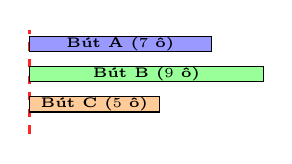
\begin{tikzpicture}[scale=0.55]
  \draw[line width=1.2pt, red!85, dashed] (0,-1.2) -- (0,1.2);
  \draw[fill=blue!40, draw=black] (0,0.7) rectangle (4.2,1.05) node[midway, font=\tiny\bfseries] {Bút A ($7$ ô)};
  \draw[fill=green!40, draw=black] (0,0) rectangle (5.4,0.35) node[midway, font=\tiny\bfseries] {Bút B ($9$ ô)};
  \draw[fill=orange!40, draw=black] (0,-0.7) rectangle (3.0,-0.35) node[midway, font=\tiny\bfseries] {Bút C ($5$ ô)};
\end{tikzpicture}
\end{center}
Xét tính đúng hoặc sai của các khẳng định sau:
\choiceTF
{\True Bút B là chiếc bút dài nhất trong ba chiếc bút.}
{\True Bút C là chiếc bút ngắn nhất trong ba chiếc bút.}
{Bút A dài hơn chiếc bút B.}
{\True Bút A dài hơn chiếc bút C.}
\loigiai{
\begin{itemize}
  \item a) \textbf{Đúng}: Bút B dài $9$ ô (dài nhất).
  \item b) \textbf{Đúng}: Bút C dài $5$ ô (ngắn nhất).
  \item c) \textbf{Sai}: Bút A ($7$ ô) ngắn hơn bút B ($9$ ô).
  \item d) \textbf{Đúng}: Bút A ($7$ ô) dài hơn bút C ($5$ ô).
\end{itemize}
}
\end{ex}

% CÂU 15: Chiều cao động vật
\begin{ex} %[1H7V25]
So sánh chiều cao của ba con vật trong vườn thú:
\begin{center}
\begin{tikzpicture}[scale=0.6]
  \draw[line width=1pt, gray!80] (-3.5,0) -- (3.5,0);
  \draw[fill=yellow!60, draw=black] (-2.5,0) rectangle (-1.7,2.8) node[midway, font=\tiny\bfseries, align=center] {Hươu\\cao cổ};
  \draw[fill=gray!40, draw=black] (-0.5,0) rectangle (0.3,1.6) node[midway, font=\tiny\bfseries, align=center] {Ngựa\\vằn};
  \draw[fill=pink!50, draw=black] (1.5,0) rectangle (2.3,0.7) node[midway, font=\tiny\bfseries, align=center] {Chú\\thỏ};
\end{tikzpicture}
\end{center}
Xét tính đúng hoặc sai của các khẳng định sau:
\choiceTF
{\True Hươu cao cổ là con vật cao nhất.}
{\True Chú thỏ là con vật thấp nhất.}
{Ngựa vằn cao hơn hươu cao cổ.}
{\True Ngựa vằn cao hơn chú thỏ.}
\loigiai{
\begin{itemize}
  \item a) \textbf{Đúng}: Hươu cao cổ cao nhất.
  \item b) \textbf{Đúng}: Chú thỏ thấp nhất.
  \item c) \textbf{Sai}: Ngựa vằn thấp hơn hươu cao cổ.
  \item d) \textbf{Đúng}: Ngựa vằn cao hơn chú thỏ.
\end{itemize}
}
\end{ex}

% CÂU 16: Đo độ dài bằng kẹp giấy
\begin{ex} %[1H7V25]
Dùng các kẹp giấy giống nhau để đo độ dài chiếc kéo và bút lông:
\begin{center}
\begin{tikzpicture}[scale=0.6]
  \node[left, font=\bfseries\tiny, color=blue!90!black] at (-0.2,0.4) {Chiếc kéo};
  \draw[fill=cyan!30, draw=black] (0,0.2) rectangle (3.2,0.6);
  \node[right, font=\bfseries\tiny] at (3.3,0.4) {($4$ kẹp giấy)};

  \node[left, font=\bfseries\tiny, color=red!90!black] at (-0.2,-0.4) {Bút lông};
  \draw[fill=red!30, draw=black] (0,-0.6) rectangle (4.0,-0.2);
  \node[right, font=\bfseries\tiny] at (4.1,-0.4) {($5$ kẹp giấy)};
\end{tikzpicture}
\end{center}
Xét tính đúng hoặc sai của các nhận xét sau:
\choiceTF
{\True Chiếc kéo dài bằng $4$ kẹp giấy.}
{\True Chiếc bút lông dài bằng $5$ kẹp giấy.}
{Chiếc kéo dài hơn chiếc bút lông.}
{\True Chiếc bút lông dài hơn chiếc kéo $1$ kẹp giấy.}
\loigiai{
\begin{itemize}
  \item a) \textbf{Đúng}: Kéo dài $4$ kẹp giấy.
  \item b) \textbf{Đúng}: Bút lông dài $5$ kẹp giấy.
  \item c) \textbf{Sai}: Chiếc kéo ngắn hơn chiếc bút lông ($4 < 5$).
  \item d) \textbf{Đúng}: $5 - 4 = 1$ kẹp giấy.
\end{itemize}
}
\end{ex}

\newpage
% --- TRANG 5: CÂU 17 ĐẾN CÂU 20 (TRẢ LỜI NGẮN / ĐIỀN SỐ) ---

\textbf{Phần 3. Trả lời ngắn}
\setcounterpageref{ex}{0}

% CÂU 17: Bút A dài hơn bút B bao nhiêu que tính
\begin{ex} %[1H7H25]
Đo bút chì $A$ và bút chì $B$ bằng que tính:
\begin{center}
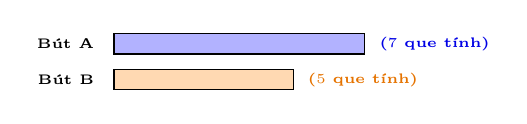
\begin{tikzpicture}[scale=0.65]
  \node[left, font=\bfseries\tiny] at (-0.2,0.35) {Bút A};
  \draw[fill=blue!30, draw=black] (0,0.15) rectangle (4.9,0.55);
  \node[right, font=\bfseries\tiny, color=blue!90!black] at (5.0,0.35) {($7$ que tính)};

  \node[left, font=\bfseries\tiny] at (-0.2,-0.35) {Bút B};
  \draw[fill=orange!30, draw=black] (0,-0.55) rectangle (3.5,-0.15);
  \node[right, font=\bfseries\tiny, color=orange!90!black] at (3.6,-0.35) {($5$ que tính)};
\end{tikzpicture}
\end{center}
Bút chì $A$ dài hơn bút chì $B$ bao nhiêu que tính?
\textit{Trả lời:} \raisebox{-2pt}{\tcbox[colframe=blue!80!black,colback=white,size=small,arc=3pt]{$2$}}
\loigiai{
Bút chì A dài hơn bút chì B số que tính là: $7 - 5 = 2$ que tính.\\
\textbf{Đáp số: $2$ que tính.}
}
\end{ex}

% CÂU 18: Sợi dây xanh ngắn hơn sợi dây đỏ bao nhiêu ô
\begin{ex} %[1H7H25]
Hai sợi dây đo trên thước kẻ ô:
\begin{center}
\begin{tikzpicture}[scale=0.65]
  \node[left, font=\bfseries\tiny] at (-0.2,0.35) {Dây đỏ};
  \draw[fill=red!40, draw=black] (0,0.15) rectangle (5.4,0.55);
  \node[right, font=\bfseries\tiny, color=red!90!black] at (5.5,0.35) {($9$ ô)};

  \node[left, font=\bfseries\tiny] at (-0.2,-0.35) {Dây xanh};
  \draw[fill=cyan!40, draw=black] (0,-0.55) rectangle (3.6,-0.15);
  \node[right, font=\bfseries\tiny, color=blue!90!black] at (3.7,-0.35) {($6$ ô)};
\end{tikzpicture}
\end{center}
Sợi dây xanh ngắn hơn sợi dây đỏ bao nhiêu ô?
\textit{Trả lời:} \raisebox{-2pt}{\tcbox[colframe=blue!80!black,colback=white,size=small,arc=3pt]{$3$}}
\loigiai{
Sợi dây xanh ngắn hơn sợi dây đỏ số ô là: $9 - 6 = 3$ ô.\\
\textbf{Đáp số: $3$ ô.}
}
\end{ex}

% CÂU 19: Bạn cao nhất trong 3 bạn
\begin{ex} %[1H7V25]
Bảng vạch chiều cao của ba bạn nhỏ:
\begin{center}
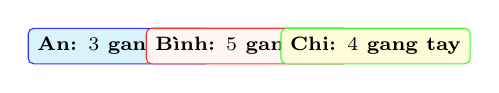
\begin{tikzpicture}[scale=0.65]
  \node[draw=blue!80, fill=cyan!15, rounded corners=2pt, font=\bfseries\scriptsize] at (-2.5,0) {An: $3$ gang tay};
  \node[draw=red!80, fill=pink!15, rounded corners=2pt, font=\bfseries\scriptsize] at (0,0) {Bình: $5$ gang tay};
  \node[draw=green!80, fill=yellow!15, rounded corners=2pt, font=\bfseries\scriptsize] at (2.5,0) {Chi: $4$ gang tay};
\end{tikzpicture}
\end{center}
Bạn cao nhất trong ba bạn là bạn nào?
\textit{Trả lời:} \raisebox{-2pt}{\tcbox[colframe=blue!80!black,colback=white,size=small,arc=3pt]{Bình}}
\loigiai{
So sánh số gang tay: $5 > 4 > 3$. Bạn cao nhất là bạn Bình.\\
\textbf{Đáp số: Bình.}
}
\end{ex}

% CÂU 20: Vận dụng cao - Ghép thêm khối lập phương để hai thanh bằng nhau
\begin{ex} %[1H7C25]
Hai thanh ghép từ các khối vuông:
\begin{center}
\begin{tikzpicture}[scale=0.6]
  % Thanh cam: 7 khối
  \node[left, font=\bfseries\tiny] at (-0.2,0.4) {Thanh cam};
  \foreach \k in {0,1,2,3,4,5,6} {
    \draw[fill=orange!50, draw=black] (\k*0.7,0.15) rectangle (\k*0.7+0.65,0.65);
  }
  \node[right, font=\bfseries\tiny, color=orange!90!black] at (5.1,0.4) {($7$ khối)};

  % Thanh xanh: 4 khối
  \node[left, font=\bfseries\tiny] at (-0.2,-0.4) {Thanh xanh};
  \foreach \k in {0,1,2,3} {
    \draw[fill=cyan!50, draw=black] (\k*0.7,-0.65) rectangle (\k*0.7+0.65,-0.15);
  }
  \node[right, font=\bfseries\tiny, color=blue!90!black] at (3.0,-0.4) {($4$ khối)};
\end{tikzpicture}
\end{center}
Cần ghép thêm bao nhiêu khối vuông vào thanh xanh để nó dài bằng thanh cam?
\textit{Trả lời:} \raisebox{-2pt}{\tcbox[colframe=blue!80!black,colback=white,size=small,arc=3pt]{$3$}}
\loigiai{
Số khối vuông cần ghép thêm vào thanh xanh là: $7 - 4 = 3$ khối.\\
\textbf{Đáp số: $3$ khối.}
}
\end{ex}
